\documentclass{beamer}

\usepackage{beamerthemebars}
\usepackage{amsmath, amssymb}
\usepackage[utf8]{inputenc}
\usepackage[ngerman]{babel}
\usepackage{url}
\usepackage{algorithm2e}
\usepackage{graphicx}
\usepackage{wrapfig}
\usepackage[font={small}]{caption}

\setbeamertemplate{footline}[frame number]
\setbeamertemplate{caption}{\raggedright\insertcaption\par}

\begin{document}

\title{Parallele Numerik - Aufgabe 1}
\author{Rebecca Seelos, Alexander Lüngen, Joshua Link}

\frame{
  \titlepage
}

\section{Aufgabe 1}
\frame{
	\frametitle{Aufgabe 1 - Teil a}
	Die Reihenfolge in welcher die IDs der Threads ausgegeben werden ist jedes Mal unterschiedlich und ist auch nicht vorherzusagen.
}
\frame{
	\frametitle{Aufgabe 1 - Teil b}
	\begin{center}
		\begin{tabular}{|l|l|r|r|r|}
			\hline
			- & Number of Threads & N & Time (s) & Speedup \\
			\hline
			sequential& 1 & $10^{7}$ & 0.239 & - \\
			& 1 & $10^{10}$ & 239.508 & - \\
			\hline
			atomic & 2 & $10^{7}$ & 0.634 & - \\
			& 4 & $10^{10}$ & $\sim$ 120 & - \\
			\hline
		\end{tabular}
	\end{center}
}

\frame{
	\frametitle{Aufgabe 1 - Teil b}
	\begin{center}
		\begin{tabular}{|l|l|r|r|r|}
			\hline
			- & Number of Threads & N & Time (s) & Speedup \\
			\hline
			sequential & 1 & $10^{7}$ & 0.239 & - \\
			& 1 & $10^{10}$ & 239.508 & - \\
			\hline
			reduction & 2 & $10^{7}$ & 0.121 & 1.9 \\
			& 2 & $10^{10}$ & 118.204 & 2 \\
			& 4 & $10^{7}$ & 0.062 & 3.9 \\
			& 4 & $10^{10}$ & 59.183 & 4 \\
			& 8 & $10^{10}$ & 29.689 & 8.0 \\
			& 16 & $10^{10}$ & 29.674 & 8.1\\
			& 32 & $10^{10}$ & 29.551 & 8.1 \\	
			\hline
		\end{tabular}
	\end{center}
}

\frame{
	\frametitle{Aufgabe 1 - Teil c}
	\begin{center}
			\begin{tabular}{|l|l|r|r|r|}
			\hline 
			Aufl"osung N & No. Threads &  Time (s) & Speedup \\
			\hline
			1000& 1 &  4.411 & - \\
			1000& 16 &  0.567 & 7.780 \\
			\hline
			2000& 1 & 17.625 & - \\
			2000& 16 &  2.248& 7.840 \\
			\hline
			4000& 1 & 71.761 & - \\
			4000& 16 &  8.980 & 7.991 \\
			\hline
			5000& 1 &  110.143 & - \\
			5000& 16 &  14.020 & 7.856\\
			\hline
		\end{tabular}
	\end{center}
}

\section{Aufgabe 2}

\frame{

	\frametitle{Aufgabe 2 - Teil a}
		\begin{enumerate}
			\item Race-Condition auf dem Array a "uber Index i
			\item Threads existieren in gesamter paralleler Region
			\item Hier ist die Variable x zunächst global definiert und wird somit implizit zwischen den Threads geshared. 
			\item f ist global definiert und wird durch jeden Thread private gesetzt. 
			\item  Race-Condition auf die Variable sum. 
		\end{enumerate} 
}

\frame{
	
	\frametitle{Aufgabe 2 - Teil b}
	\begin{itemize}
		\item Werden Matrizen in C zeilenweise im Speicher hinterlegt, ist es zur optimalen Ausnutzung von Caching-Effekten ideal, wenn auch zeilenweise über Einträge der Matrix iteriert wird.
		\item Klassischer IJK-Algorithmus: K iteriert über Spalten $\rightarrow$ Optimierung : IKJ-Algorithmus
	\end{itemize}
	
}
\frame{
	\frametitle{Aufgabe 2 - Teil b}
	\begin{center}
		\begin{tabular}{|l|p{1cm}|p{1cm}|p{1cm}|p{1.5cm}|r|r|r|r|}
			\hline
			Mode & N & Seq & \multicolumn{2}{|c|}{16 Threads} \\
			& & & Zeit & Speedup \\
			\hline
			% Methode | Problemgröße | Seq Laufzeit | 2 Threads      | 4 Threads      | 16 Threads     |
			%		  |              |              | Time | Speedup | Time | Speedup | Time | Speedup |
			gcc - IJK & 100 &           0.0190  &    0.0070  & 2.71\\
			
			gcc - IJK & 1000 &          8.8990  &    0.7240  & 12.29\\
			\hline
			gcc - IKJ & 100 &			0.0166  &        0.0060  & 2.77\\
			
			gcc - IKJ & 1000 & 			7.3744  & 	     1.6994  & 4.34\\
			\hline
			gcc - ... +Inv & 100 &	    0.0160  & 	0.0056 & 2.86\\
			gcc - ... +Inv & 1000 & 	6.0300  &	0.5086 & 11.86\\
			\hline
			gcc - ... +O2 & 100 & 0.0060  &	   0.0050  &  1.2\\
			
			gcc - ... +O2 & 1000 & 6.0412  & 	  0.5078 & 11.9\\
			\hline
		\end{tabular}
	\end{center}
	
}

\frame{
	\frametitle{Aufgabe 2 - Teil c}
	\begin{itemize}
		\item Berechnung in einigen Threads intensiver $\rightarrow$ dynamisches Scheduling führt zu optimaleren Verteilung der Arbeitslast
		\item Veränderung der chunk size hat keinen Einfluss 
	\end{itemize}

	\begin{center}
		\begin{tabular}{|p{1.5cm}|p{2cm}|p{1cm}|p{1cm}|p{1cm}|p{1cm}|p{1cm}|p{1cm}|p{1cm}|}
			\hline
			Mode & N, It., Chunk & Seq. & 8 Thr. & S.Up \\
			\hline
			static & 4000, 500, - & 34.080  &  15.061  & 2.26 \\
			static & 8000, 500, - & 135.882  &  60.522  & 2.25 \\
			\hline
			dynamic & 4000, 500, 1 & 33.955  & 4.803 & 7.07 \\
			dynamic & 8000, 500, 1 & 135.966  & 19.110 & 7.11 \\
			\hline
		\end{tabular}
	\end{center}
	
}


\section{Aufgabe 3}
\frame{
	\frametitle{Aufgabe 3 - Teil a}
	\begin{itemize}
		\item \textbf{Speedup}:  $S(n) = T(1)/T(n) $. \\ Der Zusammenhang zwischen serieller und paralleler Ausführungszeit eines Programmes. 
		\item  \textbf{Effizienz}: Die Effizienz $ E(n) = S(n)/n $ gibt die relative Verbesserung der Verarbeitungsgeschwindigkeit an.\\
		\item   \textbf{Auslastung}: $ R(n)/(n*T(n)) $. Gibt an, wie viele Operationen (Tasks) jeder Prozessor im Durchschnitt pro Zeiteinheit ausgeführt hat.\\
		\item \textbf{Mehraufwand}: $ R(n) = P(n)/P(1) $. Beschreibt den bei einem Multiprozessorsystem erforderlichen Mehraufwand für die Organisation, Synchronisation und Kommunikation der Prozessoren.\\
		\end{itemize}
		\tiny Quelle: Vorlesungsfolien Rechnerstrukturen SS2018
}

\frame{
	\frametitle{Aufgabe 3 - Teil b}
	\begin{itemize}
		\item Race-Conditions: Wenn zwei Threads unabhängig voneinander auf eine Ressource lesend oder auch schreibend zugreifen können
		\item Ungünstige Ausführungszeiten führen zu falschen Ergebnissen
		\item Um eine Race-Condition zu vermeiden, können die kritischen Abschnitte in der Art und weise gesichert werden
	\end{itemize}
}

\frame{
	\frametitle{Aufgabe 3 - Teil c}
	 \begin{tabular}{|p{2cm}|p{2.5cm}|p{2.5cm}|p{2.5cm}|}
		\hline
		- & GPUs & CPUs & FPGAs \\
		\hline
		Energieeff. & Gut & Schlecht & Gut  \\
		\hline
		Anwenderfr. & \begin{itemize}
			\item Braucht Einarbeitungszeit
			\item Es gibt Bibliotheken
		\end{itemize} & 
		\begin{itemize}
			\item Am einfachsten zu programmieren
			\item Viele Bibliotheken 
			\item Kurze Compilierzeit
		\end{itemize}  & \begin{itemize}
			\item Aufwändig zu programmieren
			\item Lange Compilierzeit
			\item Wenig Bibliotheken
		\end{itemize}  \\
		\hline
	\end{tabular}\\
	
}

\section{Aufgabe 4}
\frame{
	\frametitle{Aufgabe 4 - Teil a}
	Alle Programmdurchläufe für die Messungen hatten eine Fehlerschranke von 0.000001.\newline
	\begin{itemize}
		\item \textbf{h}: Verfeinerung $h = \frac{1}{2^l}$
		\item \textbf{l}: $l \subset \mathbb{N}$
	\end{itemize}
	\begin{center}
		\begin{tabular}{|l|l|r|r|}
			\hline
			& l=4; h=1/16 & l=5; h=1/32 & l=6; h=1/64\\
			\hline
			& 0.050s & 1.429s & 37.296s \\
			& 0.041s & 1.426s & 37.014s  \\
			& 0.040s & 1.392s & 37.061s \\
			& 0.037s & 1.428s & 37.416s  \\
			& 0.051s & 1.424s & 37.295s  \\
			\hline 
			Summe & = 0.044s & = 1.420s & = 37.216s  \\
			\hline
	
		\end{tabular}	
	\end{center}
}

\frame{
	\frametitle{Aufgabe 4 - Teil b}
	\begin{itemize}
		\item Innere Schleifendurchgänge direkt voneinander Datenabhängig
		\item Schleifen müssen in korrekter Reihenfolge abhängig von äußerer Schleife ablaufen
		\item Naive Parallelisierung der äußersten Schleife liefert falsches Ergebnis
	\end{itemize}
}

\frame{
	\frametitle{Aufgabe 4 - Teil c}
	Vorgehensweise zur optimalen Parallelisierung:
	\begin{itemize}
		\item Innere Schleifen zur Summenberechnung parallel berechnen
		\item Matrix a und Vector u explizit shared
		\item \grqq+\grqq-Reduction auf Summenvariable firstsum bzw. secondsum
	\end{itemize}

	\begin{center}
		\begin{tabular}{|l|p{2cm}|p{2cm}|r|r|}
			\hline
			&Laufzeit \-(seriell) &Laufzeit \-(parallel) & SpeedUp & Efficiency\\
			\hline
			l=4; h=1/16 & 0.044s & 0.242s & 0.182 & 0.004 \\
			l=5; h=1/32 & 1.420s & 1.154s & 1.231 & 0.026 \\
			l=6; h=1/64 & 37.216s & 26.884s & 1.384 & 0.029 \\
			\hline
		\end{tabular}
	\end{center}
}

\section{Aufgabe 5}

\frame{
	\frametitle{Aufgabe 5 - Teil a + b }
	\begin{itemize}
		\item $u$: Eine Lösung $u(x,y)$ muss mind. zweifach differenzierbar sein
		\item $f$: $f(x,y)$ muss definiert sein auf $\Omega$
		\item $\Gamma$: ist der Rand von $\Omega$ und es gilt: $\Gamma\subset\Omega $
	\end{itemize}
	\begin{center}
		Function: $f(x,y) = (N^2 + M^2)*4*\pi^2*sin(2*M*\pi*x)*sin(2*N*\pi*y)$
	\end{center}
}

\frame{
	\frametitle{Aufgabe 5 - c - Visualisiert}
	\begin{itemize}
		\item Bei der Lösungsmethodik handelt es sich um eine $h-FEM$ 
	\end{itemize}
	\begin{figure}
	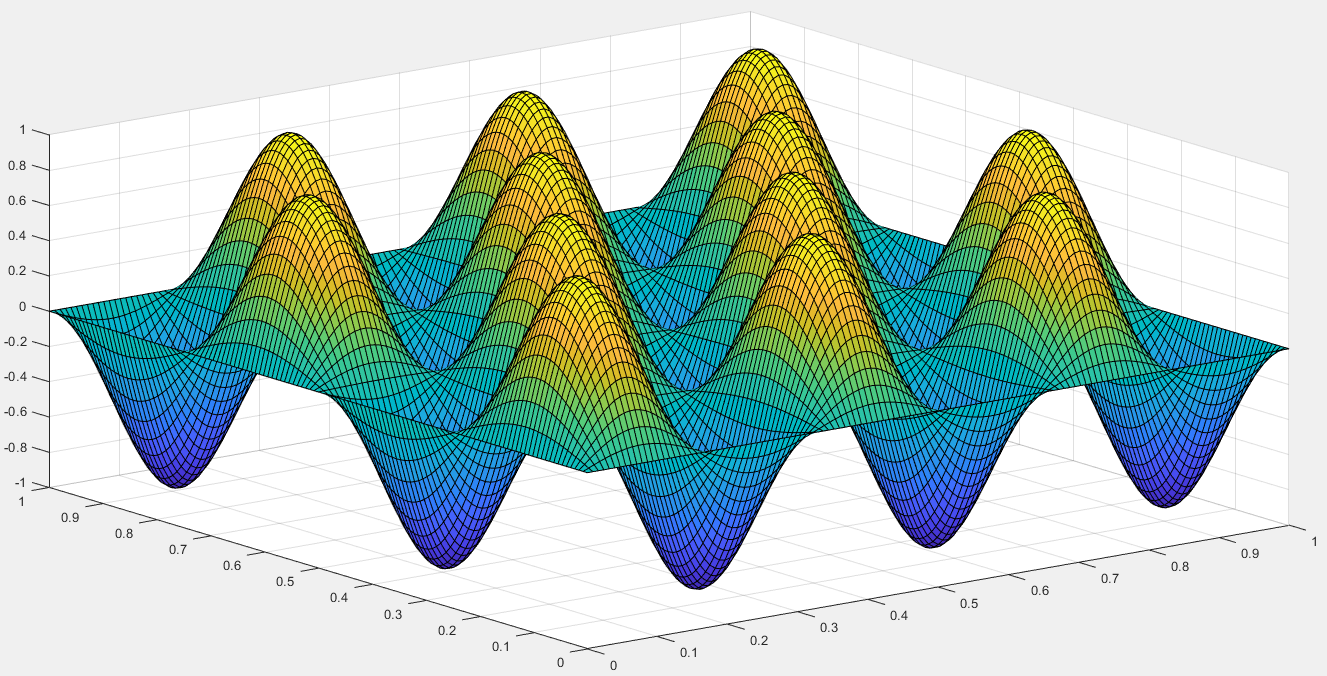
\includegraphics[width=\linewidth]{figures/A5L7M3N2.png}
		\caption{l=7; h=1/128; M=3; N=2}
	\end{figure}
}

\section{Aufgabe 6}
\frame{
	\frametitle{Aufgabe 6 - Visualisiert}
	\begin{figure}
	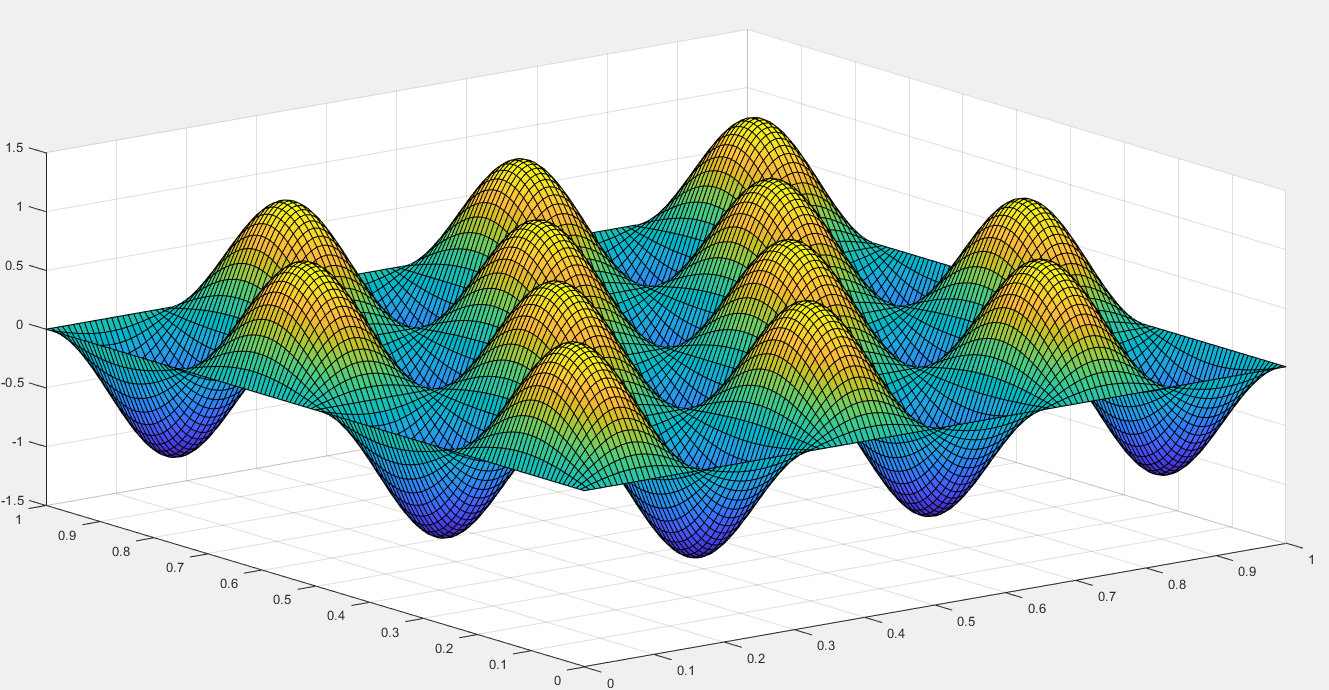
\includegraphics[width=\linewidth]{figures/A6L7M3N2.png}
		\caption{GMRES; l=7; h=1/128; M=3; N=2}
	\end{figure}
}

\frame{
	\frametitle{Aufgabe 6 - Speedup}
	\begin{tabular}{|l|l|r|r|}
		\hline
		- & Aufgabe 5(s) & Aufgabe 6(s) & Speedup\\
		\hline
		l=5; h=1/32 & 1.424 & 0.025  & 56.96 \\
		\hline
		l=6; h=1/64 & 13.276 & 0.135  & 98.488 \\
		\hline
		l=7; h=1/128 &  105.447 &  1.300  & 81.113 \\
		\hline
	\end{tabular}
}

\frame{
	\frametitle{Aufgabe 6 - Visualisiert}
	\begin{figure}
	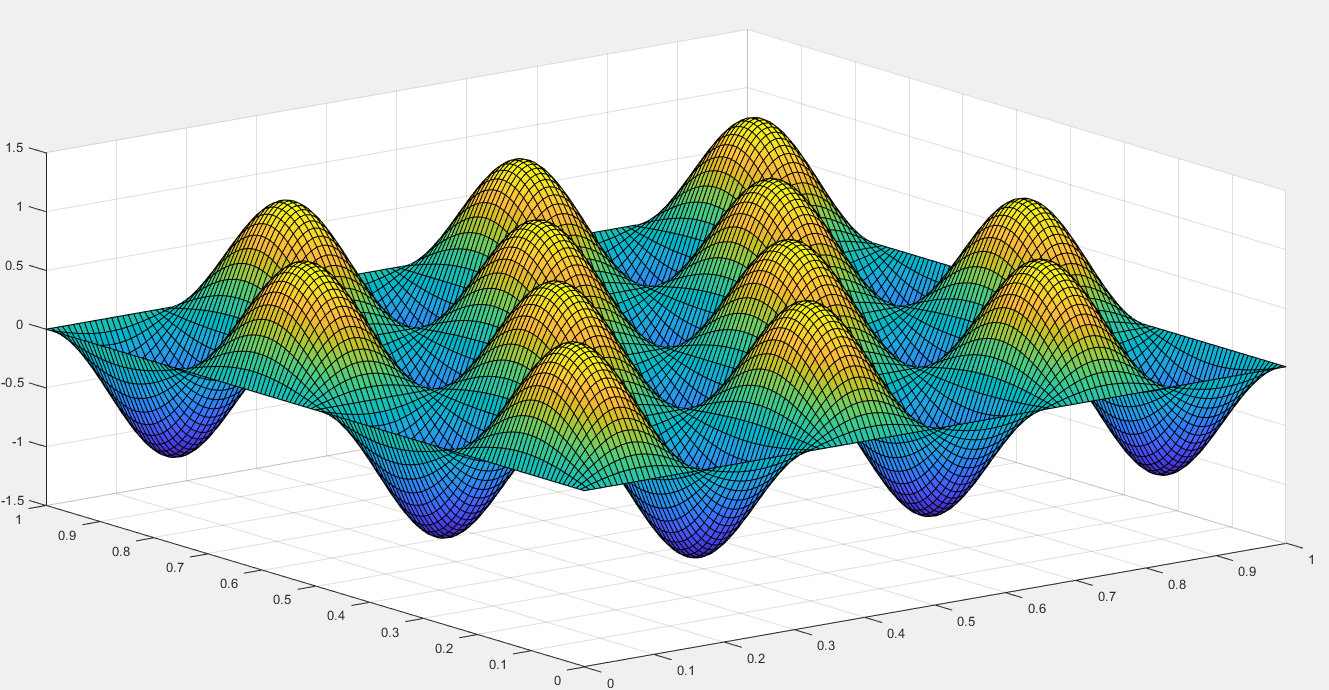
\includegraphics[width=\linewidth]{figures/A6L7M3N2.png}
		\caption{GMRES; l=7; h=1/128; M=3; N=2}
	\end{figure}
}

\section{Aufgabe 7}
\frame{
	\frametitle{Aufgabe 7}
	
}


\end{document}



%%% Local Variables: 
%%% mode: latex
%%% TeX-master: t
%%% End: 
